%qqqqqqqqqqqqqqqqqqqqqqqqqqqqqqqqqqqqqqqqqqqqqqqqqqqqqqqqqqqqqqqqqqqqqqqqq
%Quote
\begin{savequote}[50mm]
‘‘Todos los efectos de la Naturaleza son sólo la consecuencia matemática 
de un pequeño número de leyes inmutables’’
\qauthor{Pierre Simon Laplace}
\end{savequote}
%qqqqqqqqqqqqqqqqqqqqqqqqqqqqqqqqqqqqqqqqqqqqqqqqqqqqqqqqqqqqqqqqqqqqqqqqq




%#########################################################################
\chapter{Métodos Computacionales en Cosmología}
\label{cha:N-BodySimulations}


En los últimos años la física computacional ha adquirido un papel 
importante en física, permitiendo modelar diversos sistemas complejos sin
necesidad de recurrir a la experimentación u observación. Entre los métodos
abarcados por la física computacional destaca el problema de N-cuerpos 
debido a que muchos fenómenos requieren el cómputo de interacciones entre 
una gran cantidad de cuerpos, algunos ejemplos muy representativos son la 
modelación de sistemas moleculares, física de plasmas y especialmente 
problemas gravitacionales en astrofísica. El desarrollo de los métodos 
específicos para la solución de este tipo de problemas antecede la 
aparición de los ordenadores y sistemas de cómputo en general, aún así, el
desarrollo de estos potenció enormemente esta área al punto de ser la 
física computacional una nueva rama de la física.


En este capítulo se desarrollan métodos específicos para la solución de 
proble\-mas gravitacionales en astrofísica, en especial para la simulación
del universo a gran escala en régimen no lineal, partiendo de algoritmos 
básicos para el cómputo de fuerzas, métodos de detección de 
halos hasta esquemas de clasificación para el entorno cosmológico.
 

%#########################################################################




%*************************************************************************
%N-body Simulations
\section{Simulaciones de N-Cuerpos}
\label{sec:N-bodySimulations}


En general, el tipo de fenómenos más promisorios para ser modelados con 
simulaciones N-cuerpos son aquellos donde las interacciones son 
fuertemente ligadas entre las partículas, tales como fuerzas de largo 
alcance o correlaciones no locales. En la figura \ref{fig:NbodyProblem}
se ilustra un conjunto de partículas puntuales que interactúan mutuamente 
bajo alguna campo de fuerza $\bds f$, estas condiciones conforman la 
formulación clásica del problema de N-cuerpo.

\
%.........................................................................
%N-Body Problem
\begin{figure}[htbp]
	\centering
	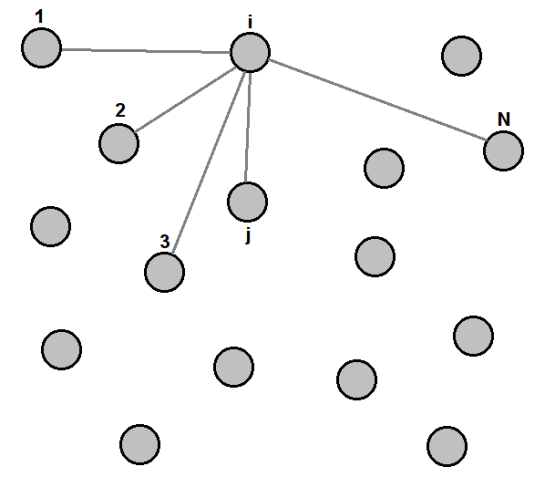
\includegraphics[width=0.50\textwidth]
	{./figures/3_nbody_simulations/Nbody_Problem.png}

	\caption{\small{Formulación del problema de N-cuerpos.}}
	
	\label{fig:NbodyProblem}
\end{figure}
%.........................................................................


Asumiendo interacciones que dependen de la posición\footnote{En el 
problema generalizado las interacciones pueden depender de otros 
parámetros tales como velocidad o grados de libertan intrínsecos como 
espín.}, la ecuación de movimiento para la partícula $i$ de la figura
\ref{fig:NbodyProblem} queda \cite{binney2008}


%.........................................................................
%Movement Equation
\eq{eq:MovementEquation}
{ \ddot{ \bds r}_i = \sum_{j=1}^N \bds f( \bds r_i, \bds r_j ) = -\nabla 
\phi( \bds r_i )\ \ \ \ \ \ \ i=1,2,\cdots,N }
%.........................................................................
donde se ha introducido la función potencial $\Phi(\bds r)$. Para el caso 
de interacción gravitacional el potencia adquiere la forma


%.........................................................................
%Gravitational Potential
\eq{eq:GravitationalPotential}
{ \phi(\bds r) = -\sum_{j=1}^N  \frac{G m_j}{|\bds r - \bds r_j|} }
%.........................................................................


La solución se obtiene a partir del conjunto $\{ \bds r_1(t),\cdots, 
\bds r_N(t) \}$ determinado a partir de las ecuaciones 
\ref{eq:MovementEquation}, para lo cual es necesario implementar 
aproximaciones numéricas debido a la no solubilidad analítica del problema.


	%---------------------------------------------------------------------
	%Direct sum
	\subsection{Método P-P}
	\label{subsec:PPMethos}
	%---------------------------------------------------------------------
	
	
La primera aproximación para la solución de las ecuaciones de movimiento
\ref{eq:MovementEquation} es computar todas las $N-1$ interacciones de la 
$i$-ésima partícula con todas las demás en un cierto tiempo $t$ y esto para 
$i=1,2,\cdots N$, luego a partir de un esquema numérico de integración se 
calculan las posiciones en un tiempo posterior discretizado $t+\Delta t$ y
así hasta un tiempo máximo $t_{\submath{max}}$ deseado. Este método
se denomina P-P (Partícula a Partícula) y es uno de los tres métodos 
estándar desarrollados para la solución del problema de N-cuerpos.


Cuando las interacciones poseen singularidades, tal como los potenciales
Coulombianos de la electrostática y la gravitación (ecuación 
\ref{eq:GravitationalPotential})


\newpage

	%---------------------------------------------------------------------
	%Tree codes
	\subsection{Códigos de Árbol}
	\label{subsec:TreeCodes}
	%---------------------------------------------------------------------


	%---------------------------------------------------------------------
	%Hidrodynamical and dark matter simulations
	\subsection{Simulaciones Hidrodinámicas y de Materia Oscura}
	\label{subsec:HidrodynamicalAndDarkMatterSimulations}
	%---------------------------------------------------------------------


%*************************************************************************




%*************************************************************************
%Types of simulations
\section{Tipos de Simulación}
\label{sec:Types of Simulations}


	%---------------------------------------------------------------------
	%Constrained simulations (CLUES)
	\subsection{Simulaciones Restringidas (CLUES)}
	\label{subsec:ConstrainedSimulations}
	%---------------------------------------------------------------------


	%---------------------------------------------------------------------
	%Unconstrained simulations (Bolshoi)
	\subsection{Simulaciones No Restringidas (Bolshoi)}
	\label{subsec:UnconstrainedSimulations}
	%---------------------------------------------------------------------


%*************************************************************************



%*************************************************************************
%Halos detection and sample definitions
\section{Detección de Halos y Definición de Muestras}
\label{sec:HalosDetectionAndSampleDefinitions}


	%---------------------------------------------------------------------
	%FOF method
	\subsection{Método FOF}
	\label{subsec:FOFMethod}
	%---------------------------------------------------------------------


	%---------------------------------------------------------------------
	%BDM method
	\subsection{Método BDM}
	\label{subsec:BDMMethod}
	%---------------------------------------------------------------------
	
	
	%---------------------------------------------------------------------
	%Sample of pairs to use
	\subsection{Muestra de Pares a Usar}
	\label{subsec:SampleOfPairsToUse}
	%---------------------------------------------------------------------
	
	
	%---------------------------------------------------------------------
	%Pair finder method
	\subsection{Método de Detección de Pares}
	\label{subsec:PairFinderMethod}
	%---------------------------------------------------------------------


%*************************************************************************




%*************************************************************************
%Environment Characterization
\section{Caracterización del Entorno}
\label{sec:EnvironmentCharacterization}


	%---------------------------------------------------------------------
	%The T-web Method
	\subsection{Método T-web}
	\label{subsec:TheT-webMethod}
	%---------------------------------------------------------------------


	%---------------------------------------------------------------------
	%The V-web Method
	\subsection{Método V-web}
	\label{subsec:TheV-webMethod}
	%---------------------------------------------------------------------


%*************************************************************************


%.........................................................................
%Curved Spaces
\begin{figure}[htbp]
	\centering
	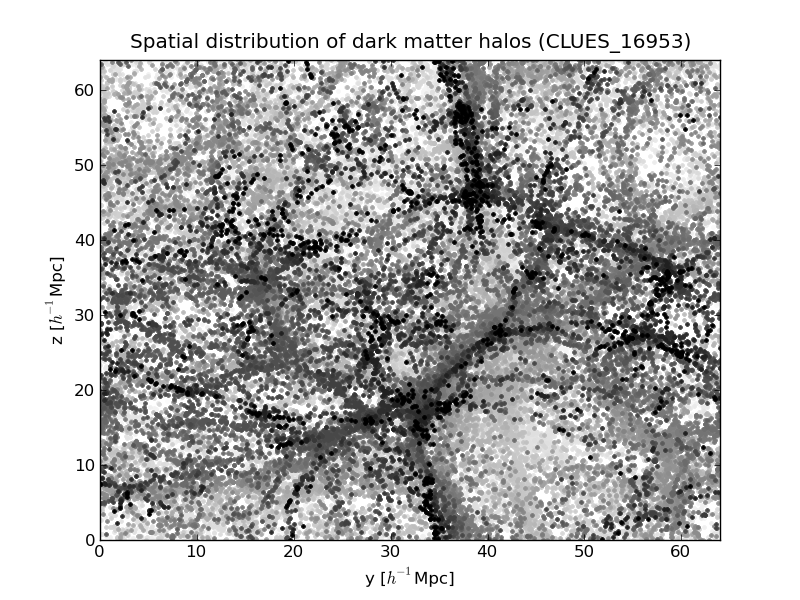
\includegraphics[width=0.49\textwidth]
	{./figures/3_nbody_simulations/Halos_Spatial_Distribution(CLUES_16953).png}
	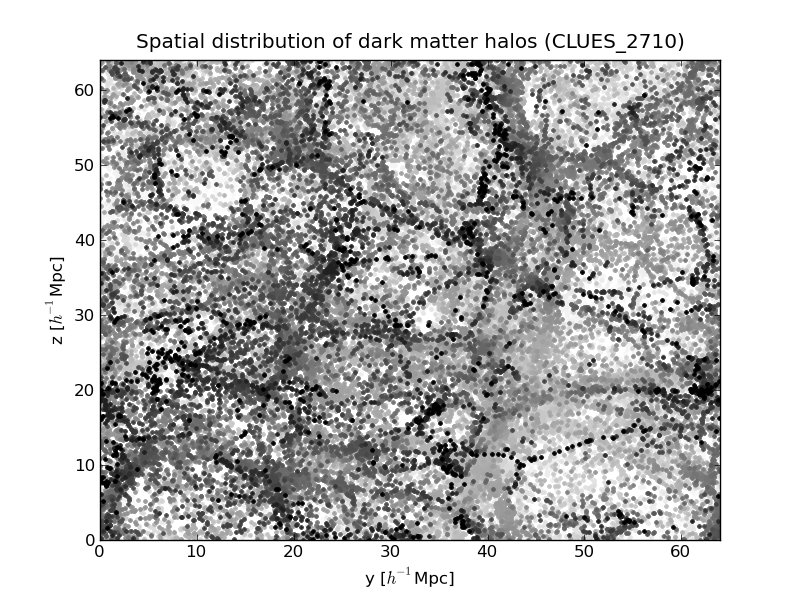
\includegraphics[width=0.49\textwidth]
	{./figures/3_nbody_simulations/Halos_Spatial_Distribution(CLUES_2710).png}
	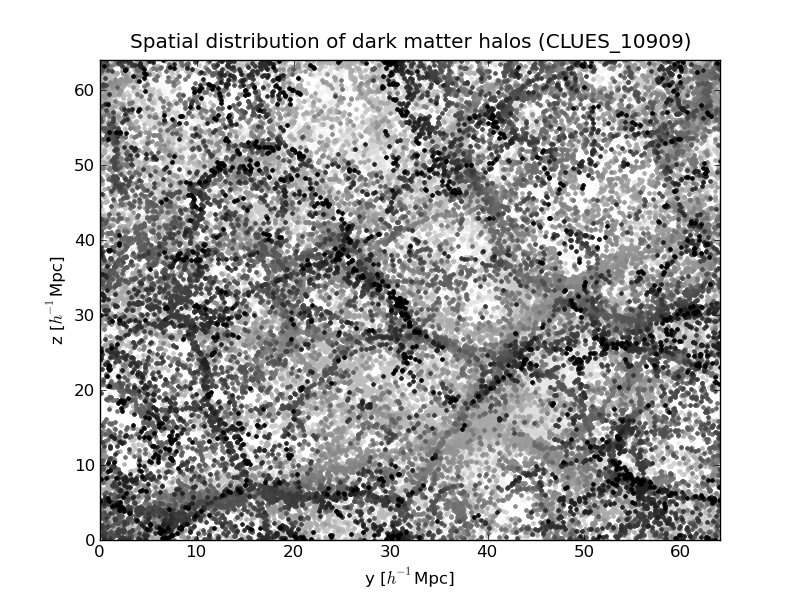
\includegraphics[width=0.49\textwidth]
	{./figures/3_nbody_simulations/Halos_Spatial_Distribution(CLUES_10909).png}

	\caption{\small{Halos en las simulaciones CLUES.}}
	
	\label{fig:CLUES}
\end{figure}
%.........................................................................